
Flow cytometry (FCM) data are multivariate measurements from flow cytometers that record light scatter and fluorescence emission properties of hundreds of thousands of individual cells. They are important to the studying of the cell structures of normal and abnormal cells and the diagnosing of human disease. \citet{cytometry_nature} introduced the FlowCAP-challenge whose main task is grouping the flow cytometry data automatically. Clustering on the FCM data is a difficult task because the distribution of the data is non-Gaussian and heavily skewed. 

We used the DLBCL Lymphoma dataset collection from~\cite{cytometry_nature} to compare our kernel algorithm with multi-view mixture of Gaussian model.
This collection of datasets contain 30 datasets, and each consists of tens of thousands of cells measurements in 5 dimensions. Each dataset is a separate clustering task, and we fit a multi-view model to each dataset separately and use the maximum-a-posteriori assignment for obtaining the cluster labels.  In each dataset, each data point is already manually labeled, and therefore we can evaluate the clustering performance using the F-score.

We splitted the 5 dimensions of the data into three views: dimension 1 and 2 as the first view, 3 and 4 the second and 5 the third view. For each dataset, we selected the best kernel bandwidth by 5-fold cross validation using log-likelihood. For EM algorithm for mixture of Gaussians (GMM) with diagonal covariances, we used a very generous 20 restarts. Figure~\ref{fig:real_data} presents the results sorted by the number of clusters. Our method (kernel spectral) outperforms EM-GMM in a majority of datasets. However, there are also datasets where kernel spectral algorithm has a large gap in performance compared to GMM. These are the datasets where the multi-view assumptions are heavily violated. Obtaining improved performance in these datasets will be a subject of our future study where we plan to develop even more robustness kernel spectral algorithms.

\begin{figure*}
  \centering
	\begin{tabular}{c}
		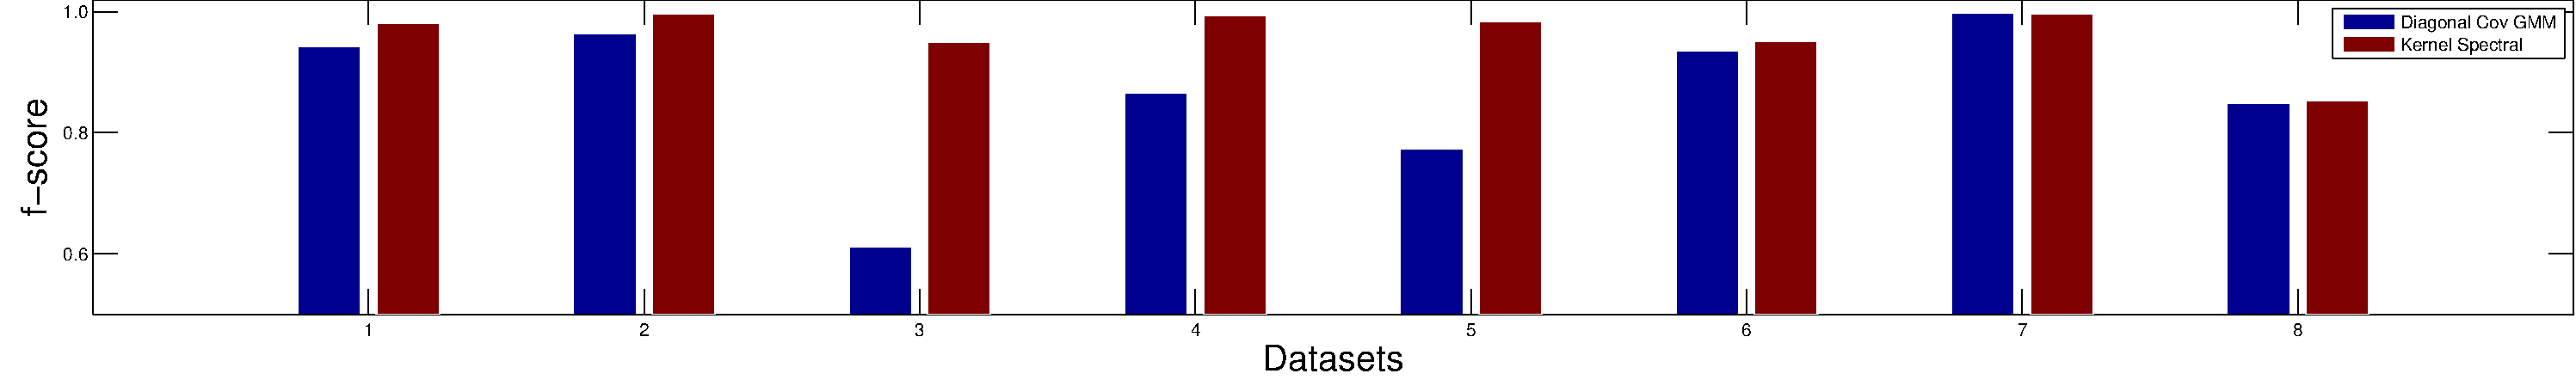
\includegraphics[width=0.82\textwidth]{../experiment/figure/paired_bar_chat_k_2} \\
		(a) number of clusters $k=2$ \\
		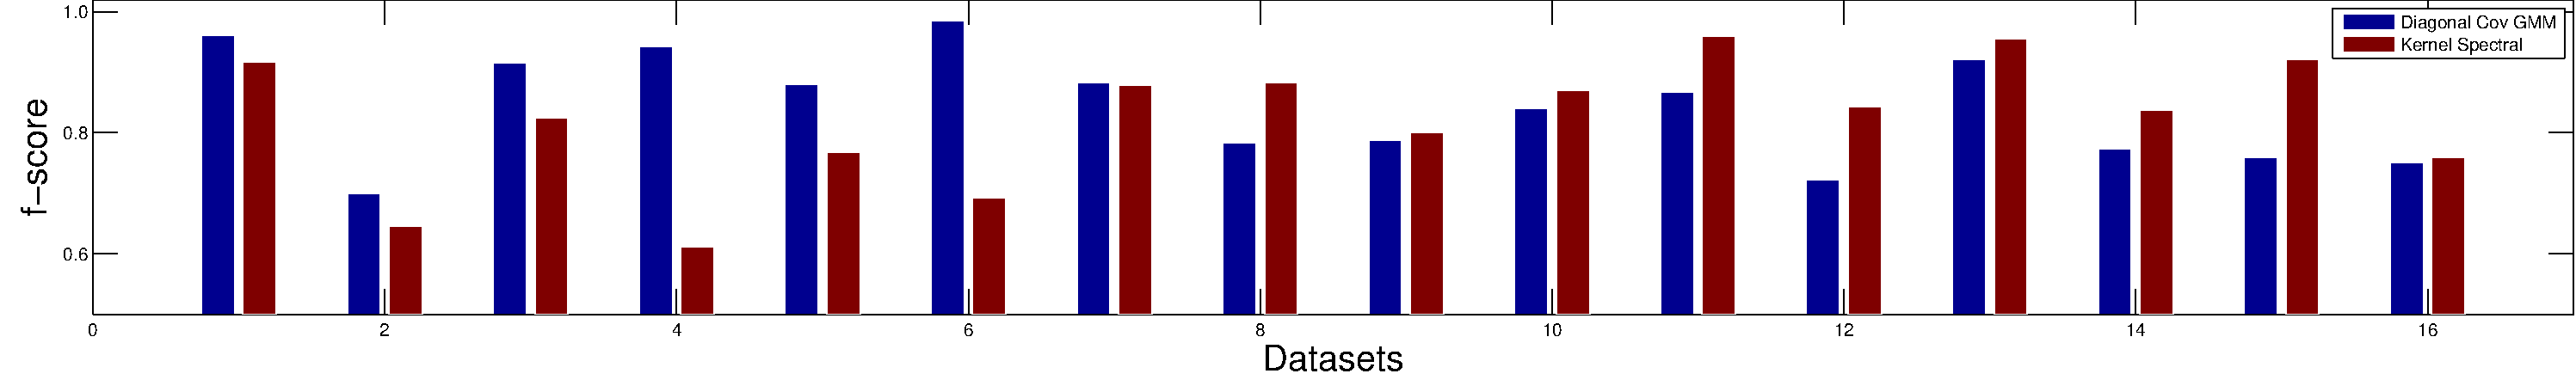
\includegraphics[width=0.98\textwidth]{../experiment/figure/paired_bar_chat_k_3}  \\
		(b) number of clusters $k=3$
	\end{tabular}
  \vspace{-3mm}
  \caption{Clustering results on DLBCL flow cytometry data. Each group of bars represents F-scores from EM-GMM with diagonal covariances~(blue) and kernel spectral method~(red). The datasets are ordered by increasing sample size.}\label{fig:real_data}
  \vspace{-3mm}
\end{figure*}
